\documentclass[../notes.tex]{subfiles}

\pagestyle{main}
\renewcommand{\chaptermark}[1]{\markboth{\chaptername\ \thechapter\ (#1)}{}}
\stepcounter{chapter}

\begin{document}




\chapter{Bonding Models}
\section{Bonding Models 1}
\begin{itemize}
    \item \marginnote{9/10:}Lecture 1 recap.
    \begin{itemize}
        \item Aspects of mechanism.
        \begin{itemize}
            \item Orbitals, energy surface, and kinetics.
            \item Masha redraws Figure \ref{fig:mechAspects}.
            \item These are the three main pictures that we'll learn about.
        \end{itemize}
        \item Today, we'll focus on orbitals.
    \end{itemize}
    \item Today: Bonding models.
    \begin{itemize}
        \item Reading: \textcite{bib:Anslyn}, Chapter 1!!
    \end{itemize}
    \item \textbf{Bonding}: How electrons are shared between nuclei.
    \begin{itemize}
        \item This determines all of molecular structure and reactivity (which is the name of this class, and underpins all of organic chemistry!).
        \item From bonding, there arise concepts such as nucleophilicity, electrophilicity, etc.
    \end{itemize}
    \item There are several levels of bonding theory / models that we'll talk about today.
    \begin{itemize}
        \item Caveat: \emph{All} of these models are no more than \emph{approximations} of reality that are useful to us.
    \end{itemize}
    \item Lecture outline.
    \begin{enumerate}
        \item Lewis structures.
        \item VSEPR.
        \item Valence Bond Theory (VBT).
        \item Molecular Orbital Theory.
        \item Qualitative Molecular Orbital Theory (QMOT).
    \end{enumerate}
    \item Lewis structures.
    \begin{figure}[h!]
        \centering
        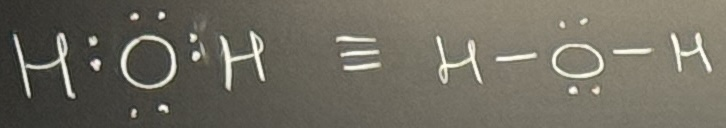
\includegraphics[width=0.2\linewidth]{LewisDots.JPG}
        \caption{Lewis dot structures.}
        \label{fig:LewisDots}
    \end{figure}
    \pagebreak
    \begin{itemize}
        \item Developed in 1916 by G. N. Lewis.
        \begin{itemize}
            \item He was nominated 48 times, but never won the Nobel Prize because some people on the review committee didn't like his "interesting personality."
        \end{itemize}
        \item In this model, we use dots to --- on paper --- indicate where electrons are in bonds.
        \item From these \textbf{Lewis dot structures}, people developed the "stick structures" that we still use today.
        \item Lewis structures are very useful in identifying the number of bonds and lone pairs.
    \end{itemize}
    \item Valence Shell Electron Pair Repulsion (VSEPR).
    \begin{itemize}
        \item Developed 1939-1957.
        \item Key finding: Electrons in bonds repel each other, so you maximize the distance between bonds.
        \item This let us go beyond Lewis structures into things like explaining tetrahedral carbon (and its \ang{109.5} bond angles).
        \item Issues develop when we try to rationalize other molecules.
        \begin{itemize}
            \item For example, isobutane has \ang{110.6} \ce{Me-C-Me} bond angles. The VSEPR purists will cite "sterics."
            \item As another example, \ce{NH3} has \ce{107} \ce{H-N-H} bond angle. The VSEPR purists will cite "lone pair is big."
        \end{itemize}
        \item Really, these were just excuses by the VSEPR purists for a bad model, and what we really needed was a new model.
    \end{itemize}
    \item Valence Bond Theory (VBT).
    \begin{itemize}
        \item Developed by Linus Pauling, with his seminal paper in 1931.
        \begin{itemize}
            \item For this work and some other stuff, he won the Nobel Prize in Chemistry in 1954.
            \item To be historically accurate, Pauling built off the work of Heitler and London (1926).
            \item However, Pauling was the person to both put everybody else's work all together and be visible enough to take the credit.
            \item Additional takeaway from Pauling's biography: Don't make your whole life about your work. For example, Pauling was shunned by many of his colleagues after he got into nuclear proliferation, but now we say he was so brave. He even won the Nobel Peace Prize!
            \item Takeaway on Pauling vs. Lewis: It pays to not be a jerk. Lewis died via cyanide poisoning (may have been an accident, but was probably suicide).
        \end{itemize}
        \item This is a quantum mechanical (QM) description of Lewis structures.
        \item Central tenet: Each atom contributes 1 valence electron in a QM-derived atomic orbital (AO).
        \begin{itemize}
            \item Shows that electrons are delocalized between atoms, and where two electrons overlap and localize is a chemical bond.
            \item In other words, electrons are not restricted to tight orbitals.
        \end{itemize}
        \item Many concepts arise within VBT until the advent of MO theory.
    \end{itemize}
    \item VBT was key for many conceptual innovations, such as \textbf{hybridization}, \textbf{electronegativity}, and \textbf{resonance}.
    \item \textbf{Hybridization}: The mixing of orbitals on the same atom to make new orbitals.
    \begin{itemize}
        \item Specifically, we can take a linear combination of AO waveforms (or AOs).
        \item More directional orbitals give you better overlap and therefore stronger bonds.
        \item Example: A linear combination $s+p_y+p_x+p_z$ yields four $sp^3$-hybridized orbitals. That's four orbitals with uneven lobes. We can draw all of these on top of each other, and from \emph{there}, we get the tetrahedral carbon.
        \item We always like new models that agree with old models; this is called a \textbf{sanity check}.
        \item We can also calculate something called the \textbf{hybridization index}.
    \end{itemize}
    \item \textbf{Hybridization index}: The number $i$ in the following formula, expressed as a function of the experimentally determined bond angle $\theta$. \emph{Denoted by} $\bm{i}$. \emph{Given by}
    \begin{equation*}
        1+i\cos\theta = 0
    \end{equation*}
    \begin{itemize}
        \item Example: \ce{NH3} has a hybridization index of 3.4.
        \item Example: \ce{H2O} has a hybridization index of 4! That's why it has the tiny bond angle. The remaining $s$-character is localized on the oxygen, and that's why we say that oxygen is electron dense and nucleophilic.
        \begin{itemize}
            \item Would this similarly predict that \ce{H2O} has longer bonds than \ce{NH3}??
        \end{itemize}
    \end{itemize}
    \item \textbf{Electronegativity}: The power of an atom to attract electrons to itself.
    \begin{itemize}
        \item There are different scales for this. We probably used the \textbf{Pauling scale}, but there is also a \textbf{Mulliken scale}.
        \item More electronegative atoms have lower energy orbitals.
        \begin{itemize}
            \item This is summarized via the \textbf{inductive effect}.
        \end{itemize}
    \end{itemize}
    \item \textbf{Inductive effect}: The withdrawing of electron density through $\sigma$-bonds.
    \begin{itemize}
        \item Example: ACN. We think about nitrogen having a partial negative charge and carbon having a partial positive charge. This results in a dipole.
        \item Takeaway: Dipoles arise from electronegativity in VBT!
    \end{itemize}
    \item \textbf{Resonance}: The superposition of several Lewis structures.
    \begin{itemize}
        \item Example: Consider an $\alpha,\beta$-unsaturated ketone. Its resonance structure is a zwitterionic intermediate, and a second resonance structure is a different zwitterion. We have three resonance forms, so that predicts more stable than something with less resonance structures. It also identifies our positive and negative reactive sites.
        \item Resonance usually happens through $\pi$-networks, but it \emph{can} happen through $\sigma$-networks.
        \item Takeaway: Delocalization of electron density leads to stability.
        \item Know your rules for drawing good resonance structures.
        \begin{itemize}
            \item We only move bonds, not atoms (no nuclear motion).
            \item Prefer to have the least separation of charge.
            \item Put the more negative charge on the more electronegative atoms.
        \end{itemize}
    \end{itemize}
    \item Limitations of VBT.
    \begin{itemize}
        \item Over time, some key experimental findings emerged that VBT coudn't explain. These results motivated people to develop a new model to explain these rare cases.
        \begin{itemize}
            \item Nowadays, exceptions to VBT are not so rare.
        \end{itemize}
        \item Remember: If a model can't explain certain cases, it's not a useful model.
        \begin{itemize}
            \item Maxim: Not predictive = not useful.
        \end{itemize}
    \end{itemize}
    \item Here's a list of the limitations of VBT.
    \begin{itemize}
        \item Doesn't account for unusual stability/instability (e.g., aromaticity and antiaromaticity).
        \item No antibonding orbitals (i.e., no explanation of interactions between molecules).
        \begin{itemize}
            \item When a nucleophile attacks a ketone, the interaction is with the antibonding orbital of the ketone. Forming a new bond involves populating an antibonding orbital.
        \end{itemize}
        \item Thursday is all about aromaticity, and modern ways to conceptualize it.
    \end{itemize}
    \pagebreak
    \item This leads to the mother of all bonding models, Molecular Orbital Theory.
    \begin{itemize}
        \item Central tenet: Molecular orbitals (e.g., $\sigma$, $\sigma^*$, $\pi$, $\pi^*$) arise from linear combinations of atomic orbitals (in Orgo, this is $s$ \& $p$; we won't consider $d$-orbital effects so much).
        \item We consider the electronic structure of the whole molecule, not just atoms or bonds.
        \begin{itemize}
            \item We focus on key molecular orbitals such as the HOMO and LUMO.
        \end{itemize}
        \item We also get \textbf{group orbitals}: Leads into QMOT, which is MOs for prototypical groups.
    \end{itemize}
    \item MO theory leads to MO diagrams.
    \begin{figure}[h!]
        \centering
        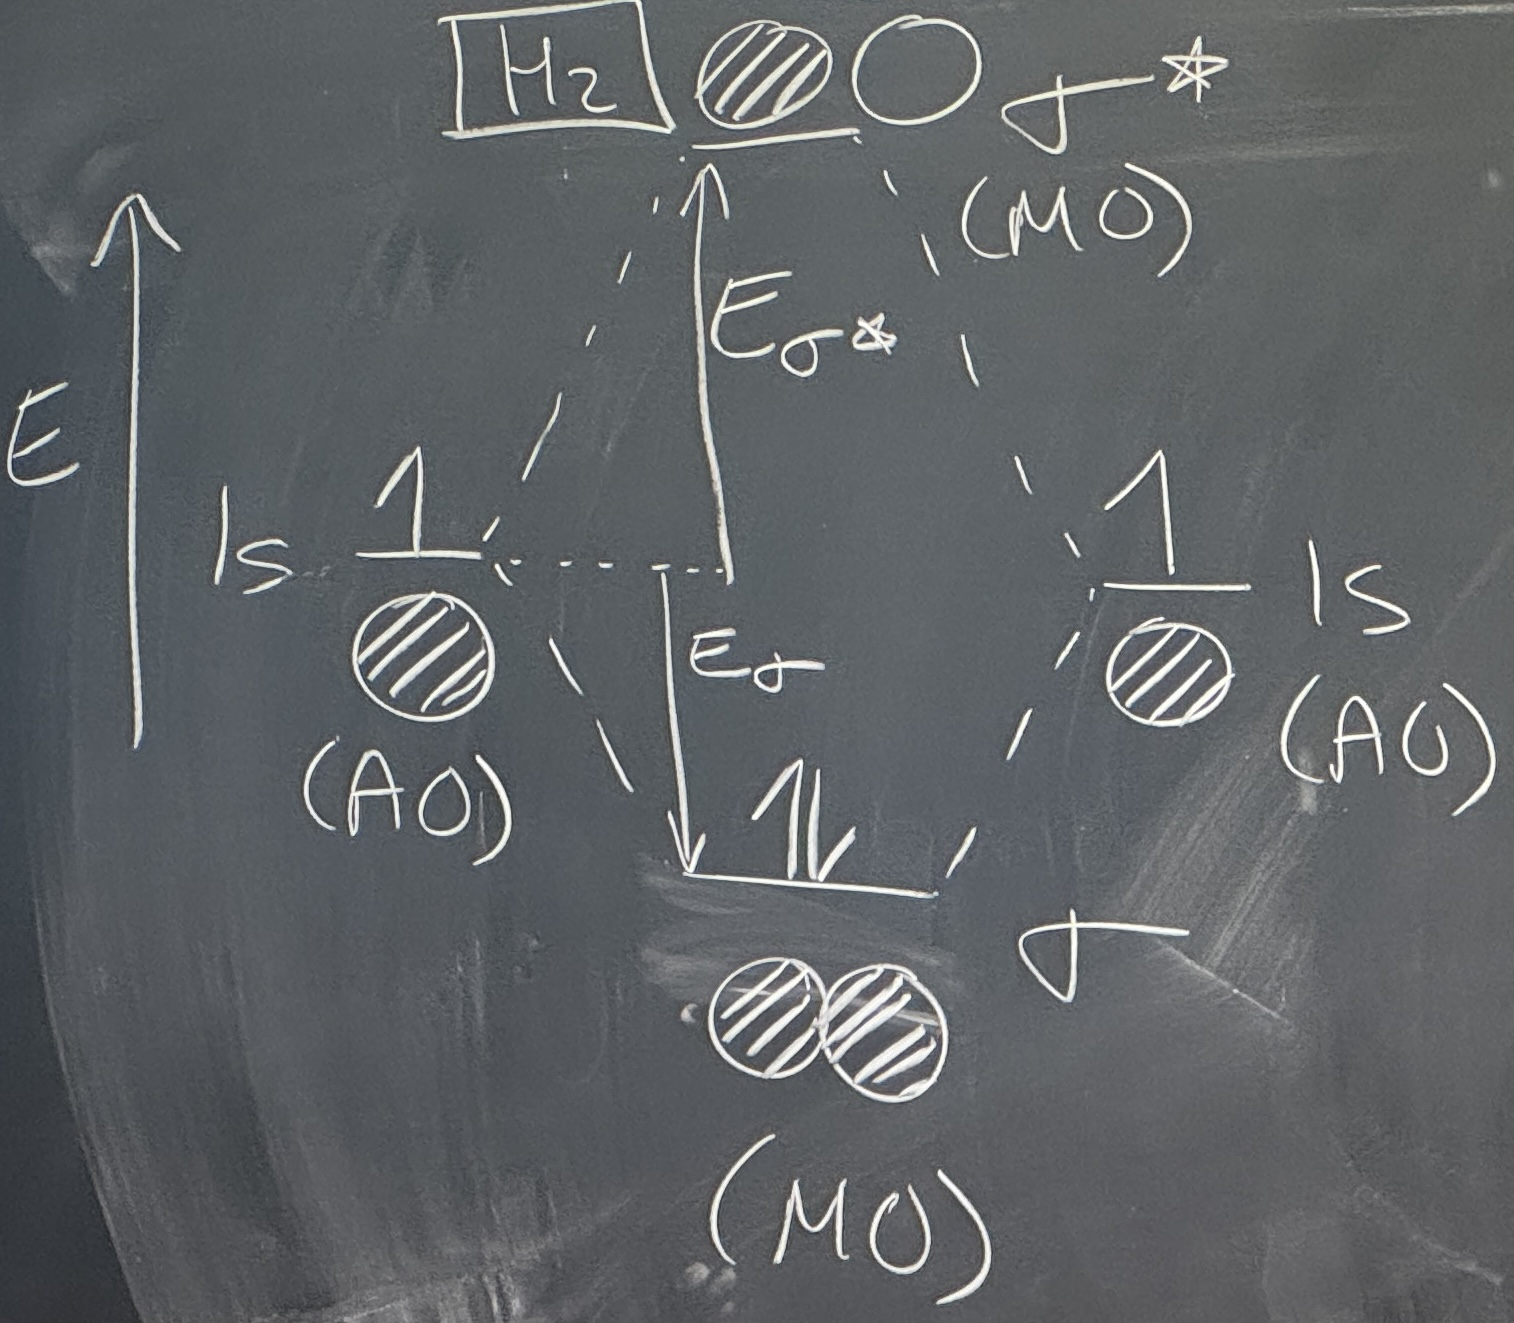
\includegraphics[width=0.3\linewidth]{MOH2.JPG}
        \caption{MO diagram for \ce{H2}.}
        \label{fig:MOH2}
    \end{figure}
    \begin{itemize}
        \item Two atomic orbitals interact to fill two molecular orbitals.
        \item We fill the bonding orbital with all the electrons that come in (in this case, 2).
        \item The energy of stabilization is $E_{\sigma}$.
        \item The destabilization energy is $E_{\sigma^*}$.
        \item Read \textcite{bib:Anslyn} for more rules.
        \item Notes.
        \begin{itemize}
            \item $|E_{\sigma^*}|>|E_{\sigma}|$. Thus, if the antibonding orbitals get populated, the moleucle breaks. This is because of nuclear repulsion.
            \item The $\sigma$-bond is more stable than the $1s$ orbitals by themselves. This is why the \ce{H-H} bond forms. This kind of analysis allows us to predict whether or not a bond will form.
        \end{itemize}
        \item Question for us to consider: Why doesn't \ce{He-He} form?
        \begin{itemize}
            \item Because its antibonding MOs would be populated.
        \end{itemize}
    \end{itemize}
    \item Example MO diagram: Ethylene.
    \begin{figure}[H]
        \centering
        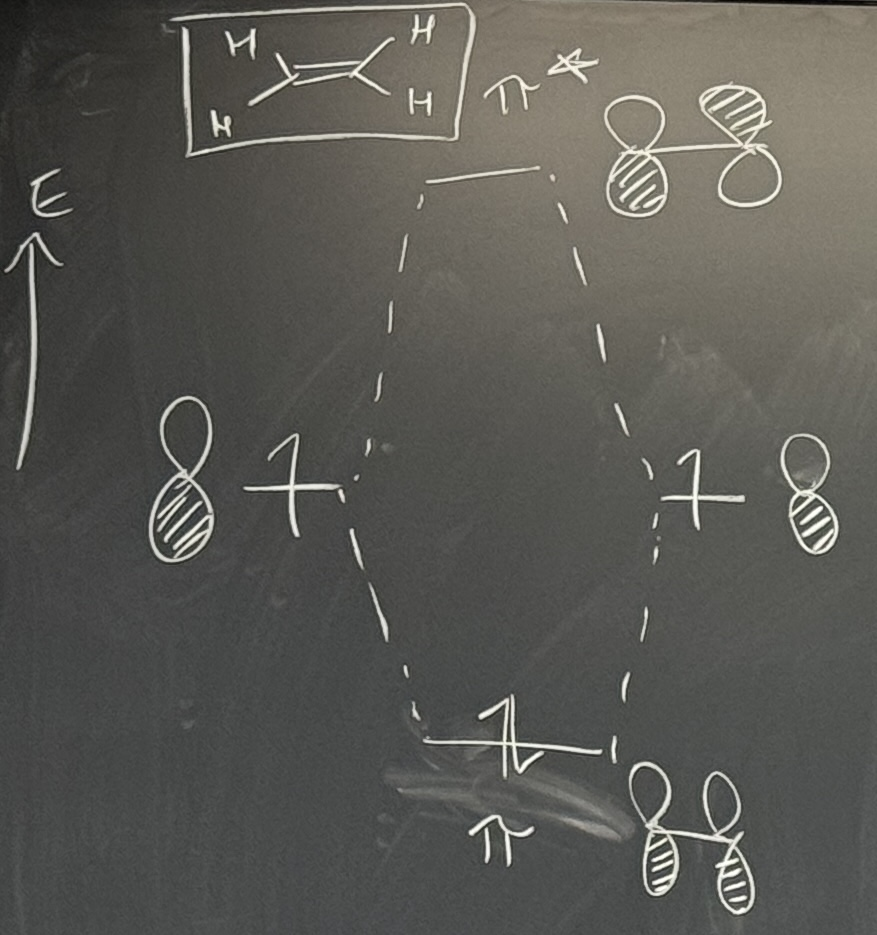
\includegraphics[width=0.3\linewidth]{MOEtH.JPG}
        \caption{MO diagram for ethylene.}
        \label{fig:MOEtH}
    \end{figure}
    \begin{itemize}
        \item Looking specifically at the $\pi$-bond formation.
        \item This is why we form a stable $\pi$-bond.
    \end{itemize}
    \item Example MO diagram: Formaldehyde.
    \begin{figure}[h!]
        \centering
        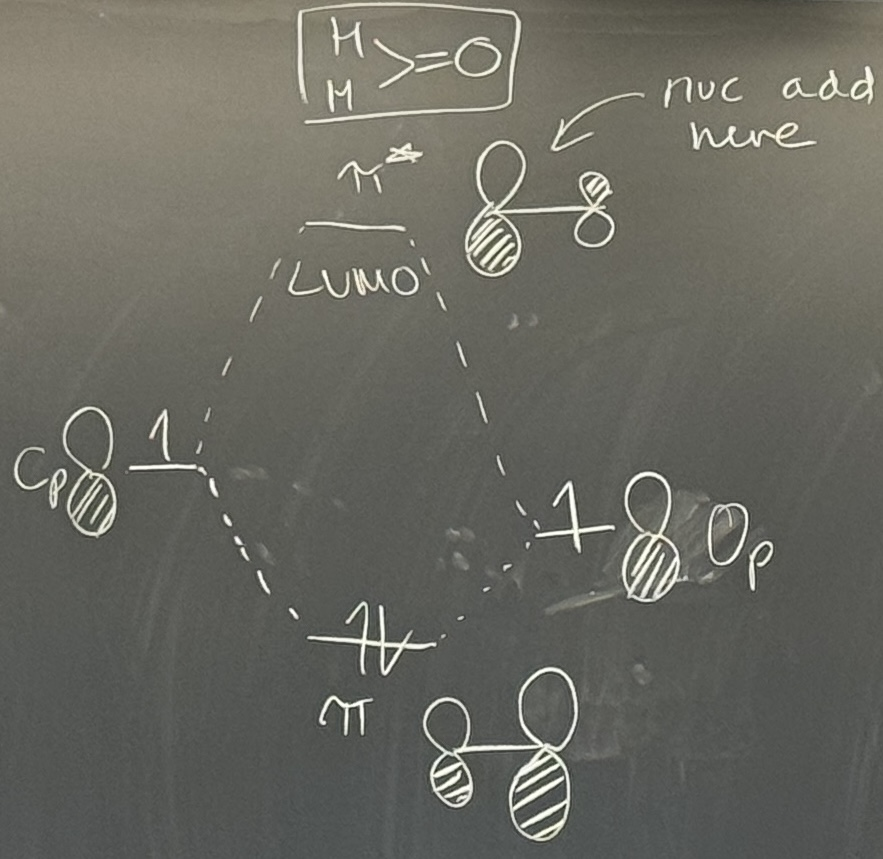
\includegraphics[width=0.3\linewidth]{MOForm.JPG}
        \caption{MO diagram for formaldehyde.}
        \label{fig:MOForm}
    \end{figure}
    \begin{itemize}
        \item We mix a \ce{C_{$p$}} AO and a (lower energy) \ce{O_{$p$}} AO.
        \item These orbitals interact less well than those in ethylene due to their difference in energy.
        \item We benefit from constructive phasing, but the lobes are much bigger on oxygen.
        \item In the antibonding orbital, the lobes are much bigger on carbon.
        \item Principles revealed by this MO diagram.
        \begin{itemize}
            \item Closer energy AOs give stronger mixing, resulting in lower energy MOs. Lower energy MOs are more stabilizing.
            \item More electronegative atoms have lower energy atomic orbitals.
            \item The $\pi$-orbital is asymmetric because its energetically more similar to \ce{O_{$p$}} than \ce{C_{$p$}}.
            \begin{itemize}
                \item In other words, it's going to look more like the \ce{O_{$p$}} orbital.
                \item One more way of stating this is that the coefficient of oxygen in the LCAO is bigger.
            \end{itemize}
        \end{itemize}
        \item We know that the LUMO (frontier orbital) interacts with nucleophiles. The lobe of the LUMO is bigger on carbon, hence why we react there.
    \end{itemize}
    \item Qualitative MO theory (QMOT).
    \begin{itemize}
        \item All about forming group orbitals for common functional groups or motifs.
        \item Essentially, we may not need to calculate MOs for the whole molecule to find out how every carbonyl reacts; we can trust that carbonyl group orbitals are decently conserved.
        \item There are a bunch of rules for how to form a QMOT diagram.
        \begin{itemize}
            \item See Table 1.7 in \textcite{bib:Anslyn} for building QMOT diagrams.
        \end{itemize}
        \item This is the basis of \textbf{Walsh diagrams}.
        \item We can build group MOs from linear combinations of $s$ \& $p$ AOs.
    \end{itemize}
    \item \textbf{Walsh diagram}: A representation of an MO diagram as a function of geometric distortions.
    \begin{itemize}
        \item This matters because geometry affects orbital overlap, which can be destabilizing or stabilizing.
    \end{itemize}
    \pagebreak
    \item Example QMOT diagram: \ce{CH3}.
    \begin{figure}[h!]
        \centering
        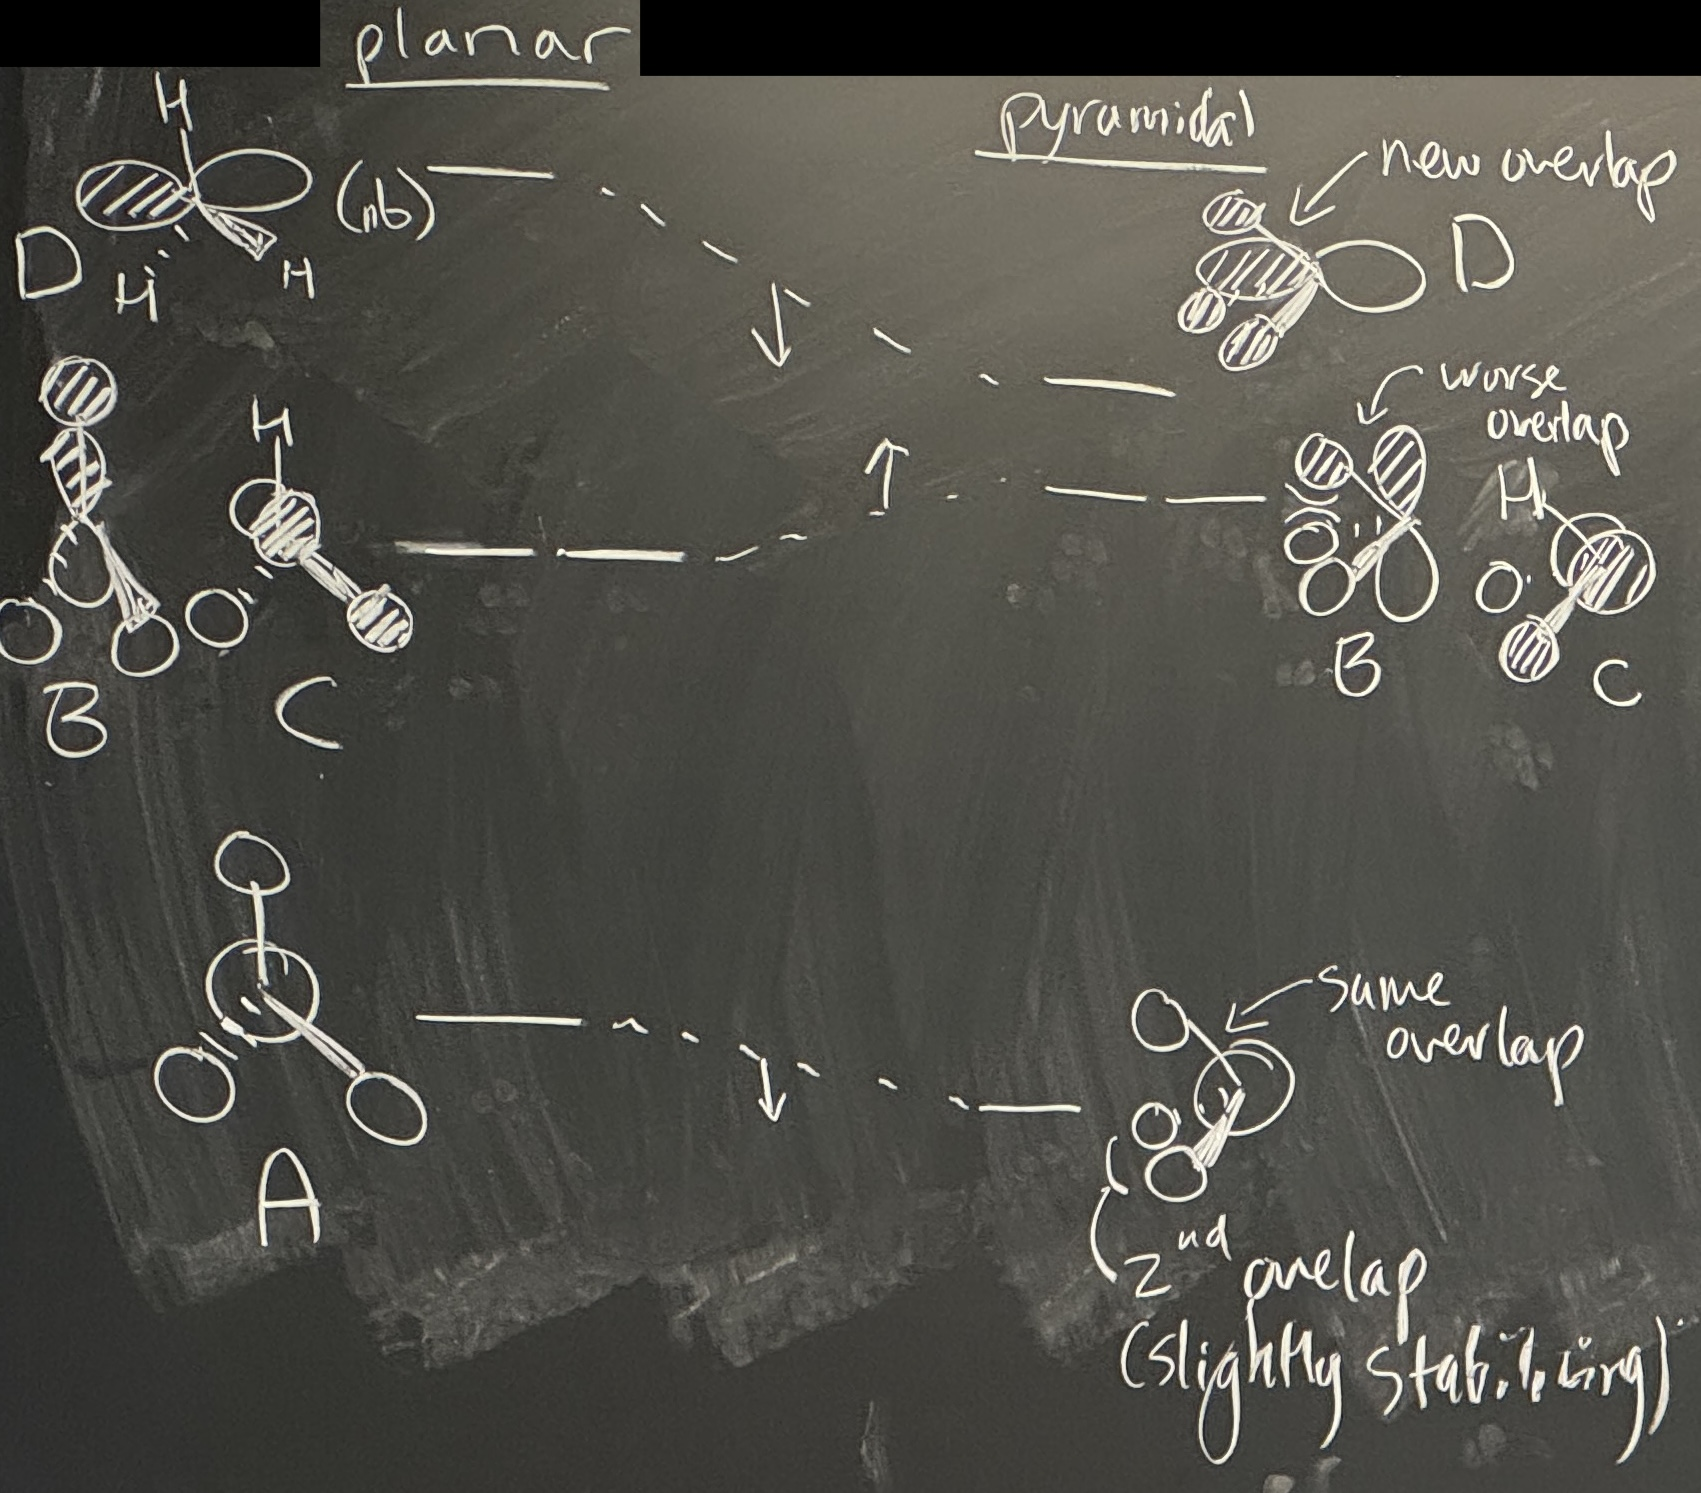
\includegraphics[width=0.4\linewidth]{QmotCH3.JPG}
        \caption{QMOT diagram for \ce{CH3}.}
        \label{fig:QmotCH3}
    \end{figure}
    \begin{itemize}
        \item Key question: What geometry of \ce{CH3} is favorable?
        \item Masha defines axes.
        \item Undetermined yet if this is a radical, cation, or anion. We'll get there!
        \item We look at a planar set of orbitals first.
        \begin{enumerate}[label={\textbf{\Alph*}.}]
            \item All phases in sync, all $s$ orbitals.
            \item Phases align top to bottom with the $p_x$ orbital of carbon.
            \item Phases align in and out of the board with the $p_y$ orbital of carbon.
            \item Nonbonding; just the $p_z$ orbital.
        \end{enumerate}
        \item There are also \textbf{E}, \textbf{F}, and \textbf{G} orbitals that are energetically above these, but we won't draw them for now (because we won't fill them with electrons in the carbocation, carbanion, or carbon radical).
        \begin{itemize}
            \item The \textbf{E}, \textbf{F}, and \textbf{G} orbitals will have the opposite phasing of the lower orbitals!
        \end{itemize}
        \item We now draw an analogous, pyramidal set of orbitals.
        \begin{enumerate}[label={\textbf{\Alph*}.}]
            \item Overlap is \emph{slightly} more favorable because we have a secondary orbital interaction between the hydrogens now. The \ce{C-H} overlap stays the same.
            \item Worse overlap. We're losing a \textbf{primary} interaction instead of gaining a \textbf{secondary} one, so the energy of \textbf{B} actually goes up \emph{more} than \textbf{A} went down. We also get some destabilizing secondary interaction between the \ce{H} orbitals.
            \item Just like \textbf{B}, we get worse primary overlap, and new interfering secondary overlap.
            \item Gets stabilized the \emph{most} significantly! This is because we've taken something with no bonding interactions and \emph{created} bonding interactions between the $p$-orbital and the hydrogens.
        \end{enumerate}
        \item Relationship between QMOT and Walsh diagrams: A Walsh diagram is a QMOT diagram with everything connected.
        \item Now how do we fill electrons?
        \begin{itemize}
            \item Consider the \ce{CH3+} cation: We have 6 electrons, so we populate the planar orbitals because it's more stable overall.
            \item Consider the \ce{CH3-} anion: We have 8 electrons, so we populate the pyramidal orbitals because \emph{they're} more stable overall.
        \end{itemize}
        \item This rigorous prediction of conformation is the benefit of this model.
        \item We can also use this model for other isostructural molecules.
        \pagebreak
        \item Examples.
        \begin{itemize}
            \item \ce{NH3}: 8 electrons, pyramidal.
            \item \ce{BH3}: 6 electrons, planar.
            \item \ce{*CH3}: 7 electrons, \emph{slightly} planar.
            \begin{itemize}
                \item But this is a special case only for \ce{*CH3}; any other radical is pyramidal.
            \end{itemize}
        \end{itemize}
    \end{itemize}
    \item \textbf{Primary} (orbital interaction): An interaction between orbitals on adjacent atoms in a molecule.
    \item \textbf{Secondary} (orbital interaction): An interaction between orbitals on atoms that are separated by one other atom in a molecule.
    \item What is quantitative about QMOT?
    \begin{itemize}
        \item There is a lot more depth in \textcite{bib:Anslyn}. You can calculate the actual potential energy surface and figure out these conformations exactly.
    \end{itemize}
    \item Example QMOT diagram: \ce{CH2}.
    \begin{figure}[h!]
        \centering
        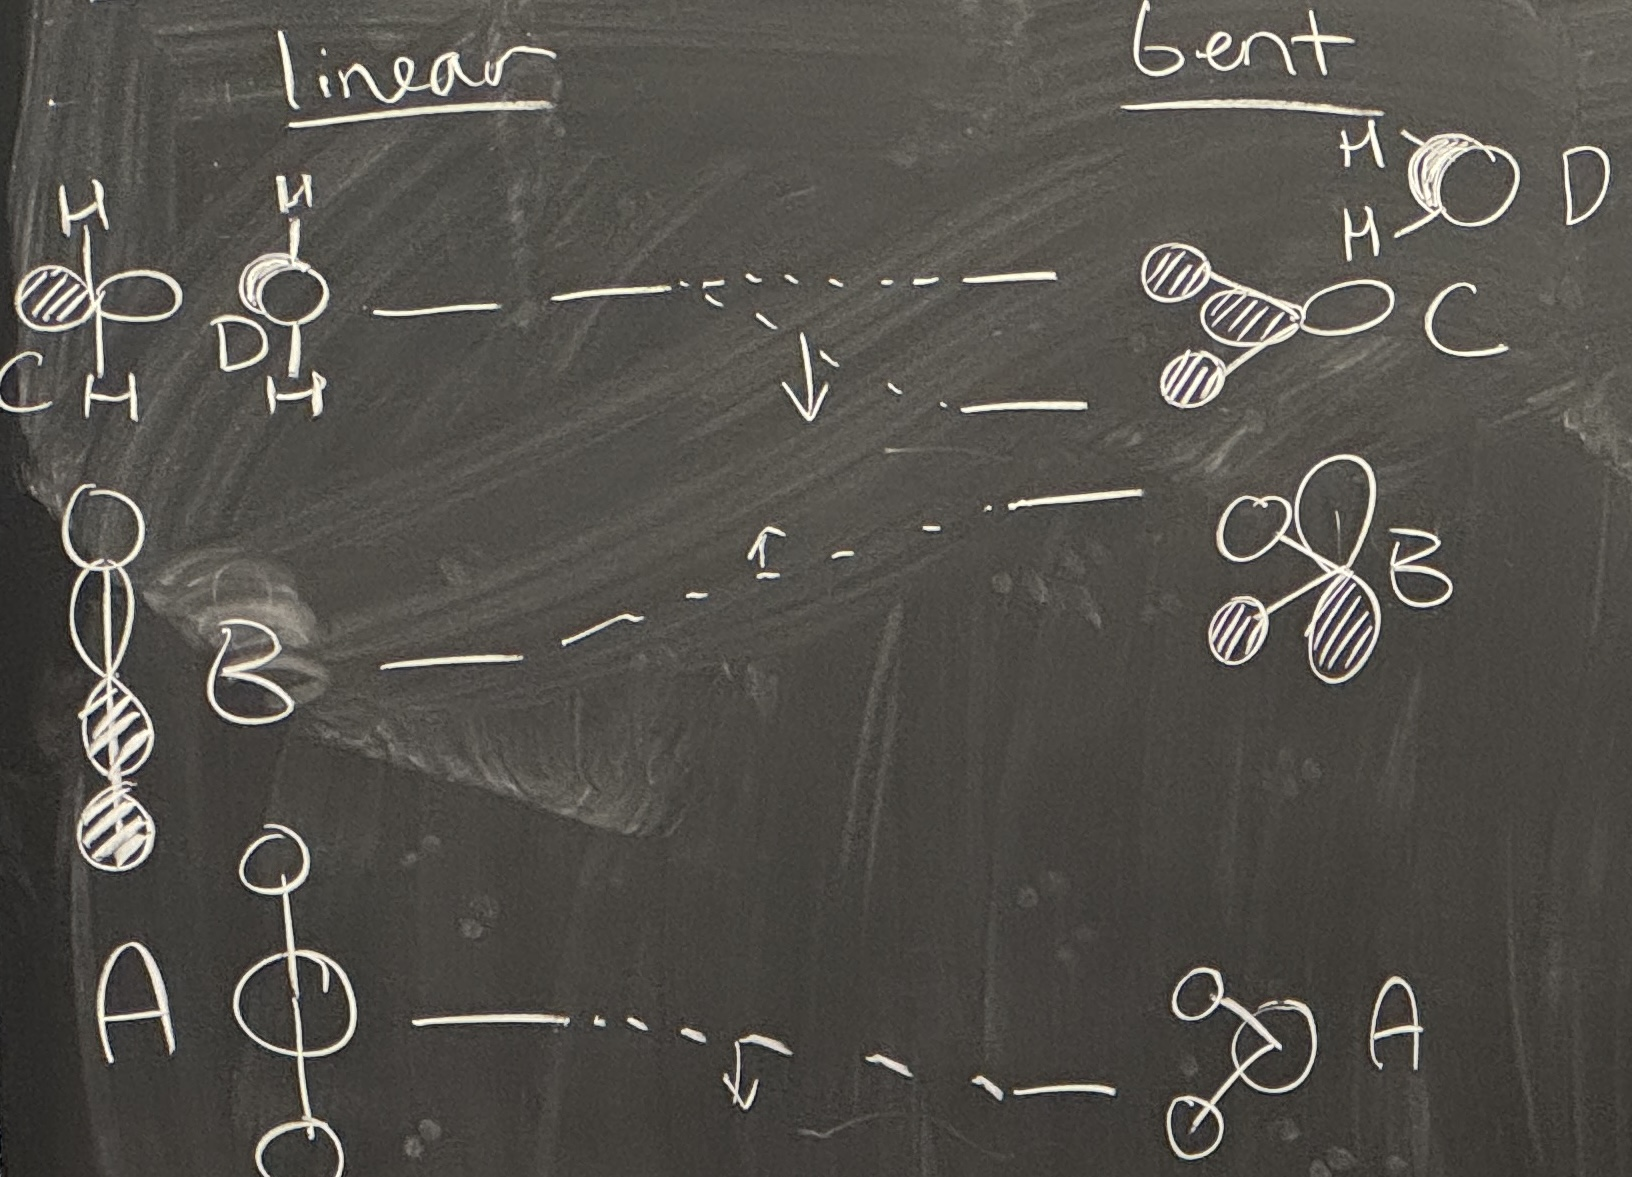
\includegraphics[width=0.4\linewidth]{QmotCH2.JPG}
        \caption{QMOT diagram for \ce{CH2}.}
        \label{fig:QmotCH2}
    \end{figure}
    \begin{itemize}
        \item Two geometries: Linear and bent.
        \item Linear.
        \begin{enumerate}[label={\textbf{\Alph*}.}]
            \item Linear chain of $s$-orbitals with matching phases.
            \item Linear chain of matching phases orbitals, with $p_x$ on carbon.
            \item One of the other $p$-orbitals, with no phasing.
            \item The last remaining $p$-orbital, again with no phasing.
        \end{enumerate}
        \item Bent.
        \begin{enumerate}[label={\textbf{\Alph*}.}]
            \item Goes down slightly. We kept primary, and added secondary.
            \item Losing primary overlap and gaining a destabilizing secondary interaction; higher $E$ like before.
            \item Adding \emph{significant} constructive interference. Biggest effect again!
            \item Staying the same; no bonding interactions to begin or end with. We don't consider secondary interactions when there's no density at all there.
        \end{enumerate}
        \item Example species.
        \begin{itemize}
            \item \ce{H2O}: 8 electrons, bent.
            \begin{itemize}
                \item Note that this model predicts that \ce{H2O} has nondegenerate lone pairs, which has been experimentally verified!
                \item Bulk water acts as if it has degenerate lone pairs. We can read \textcite{bib:Anslyn} about this, but otherwise, it's outside the scope of the class.
            \end{itemize}
            \pagebreak
            \item \ce{CH2} (a \textbf{carbene}): 6 electrons, a mix of linear and bent!
            \begin{itemize}
                \item We'll return to carbenes in a few weeks.
                \item We'll define \textbf{triplet} (2 electrons in different orbitals) and \textbf{singlet} (2 electrons in same orbital) carbenes later.
                \item Triplet is \ang{136}, and singlet is \ang{105}, so the triplet is more linear and the singlet is more bent! The triplet has reactivity more characteristic of the linear orbital picture, and the singlet has reactivity more characteristic of the bent orbital picture.
                \item The triplet is more favored by \SI[per-mode=symbol]{9}{\kilo\calorie\per\mole}
            \end{itemize}
        \end{itemize}
    \end{itemize}
    \item Example QMOT diagram: Formaldehyde.
    \begin{figure}[h!]
        \centering
        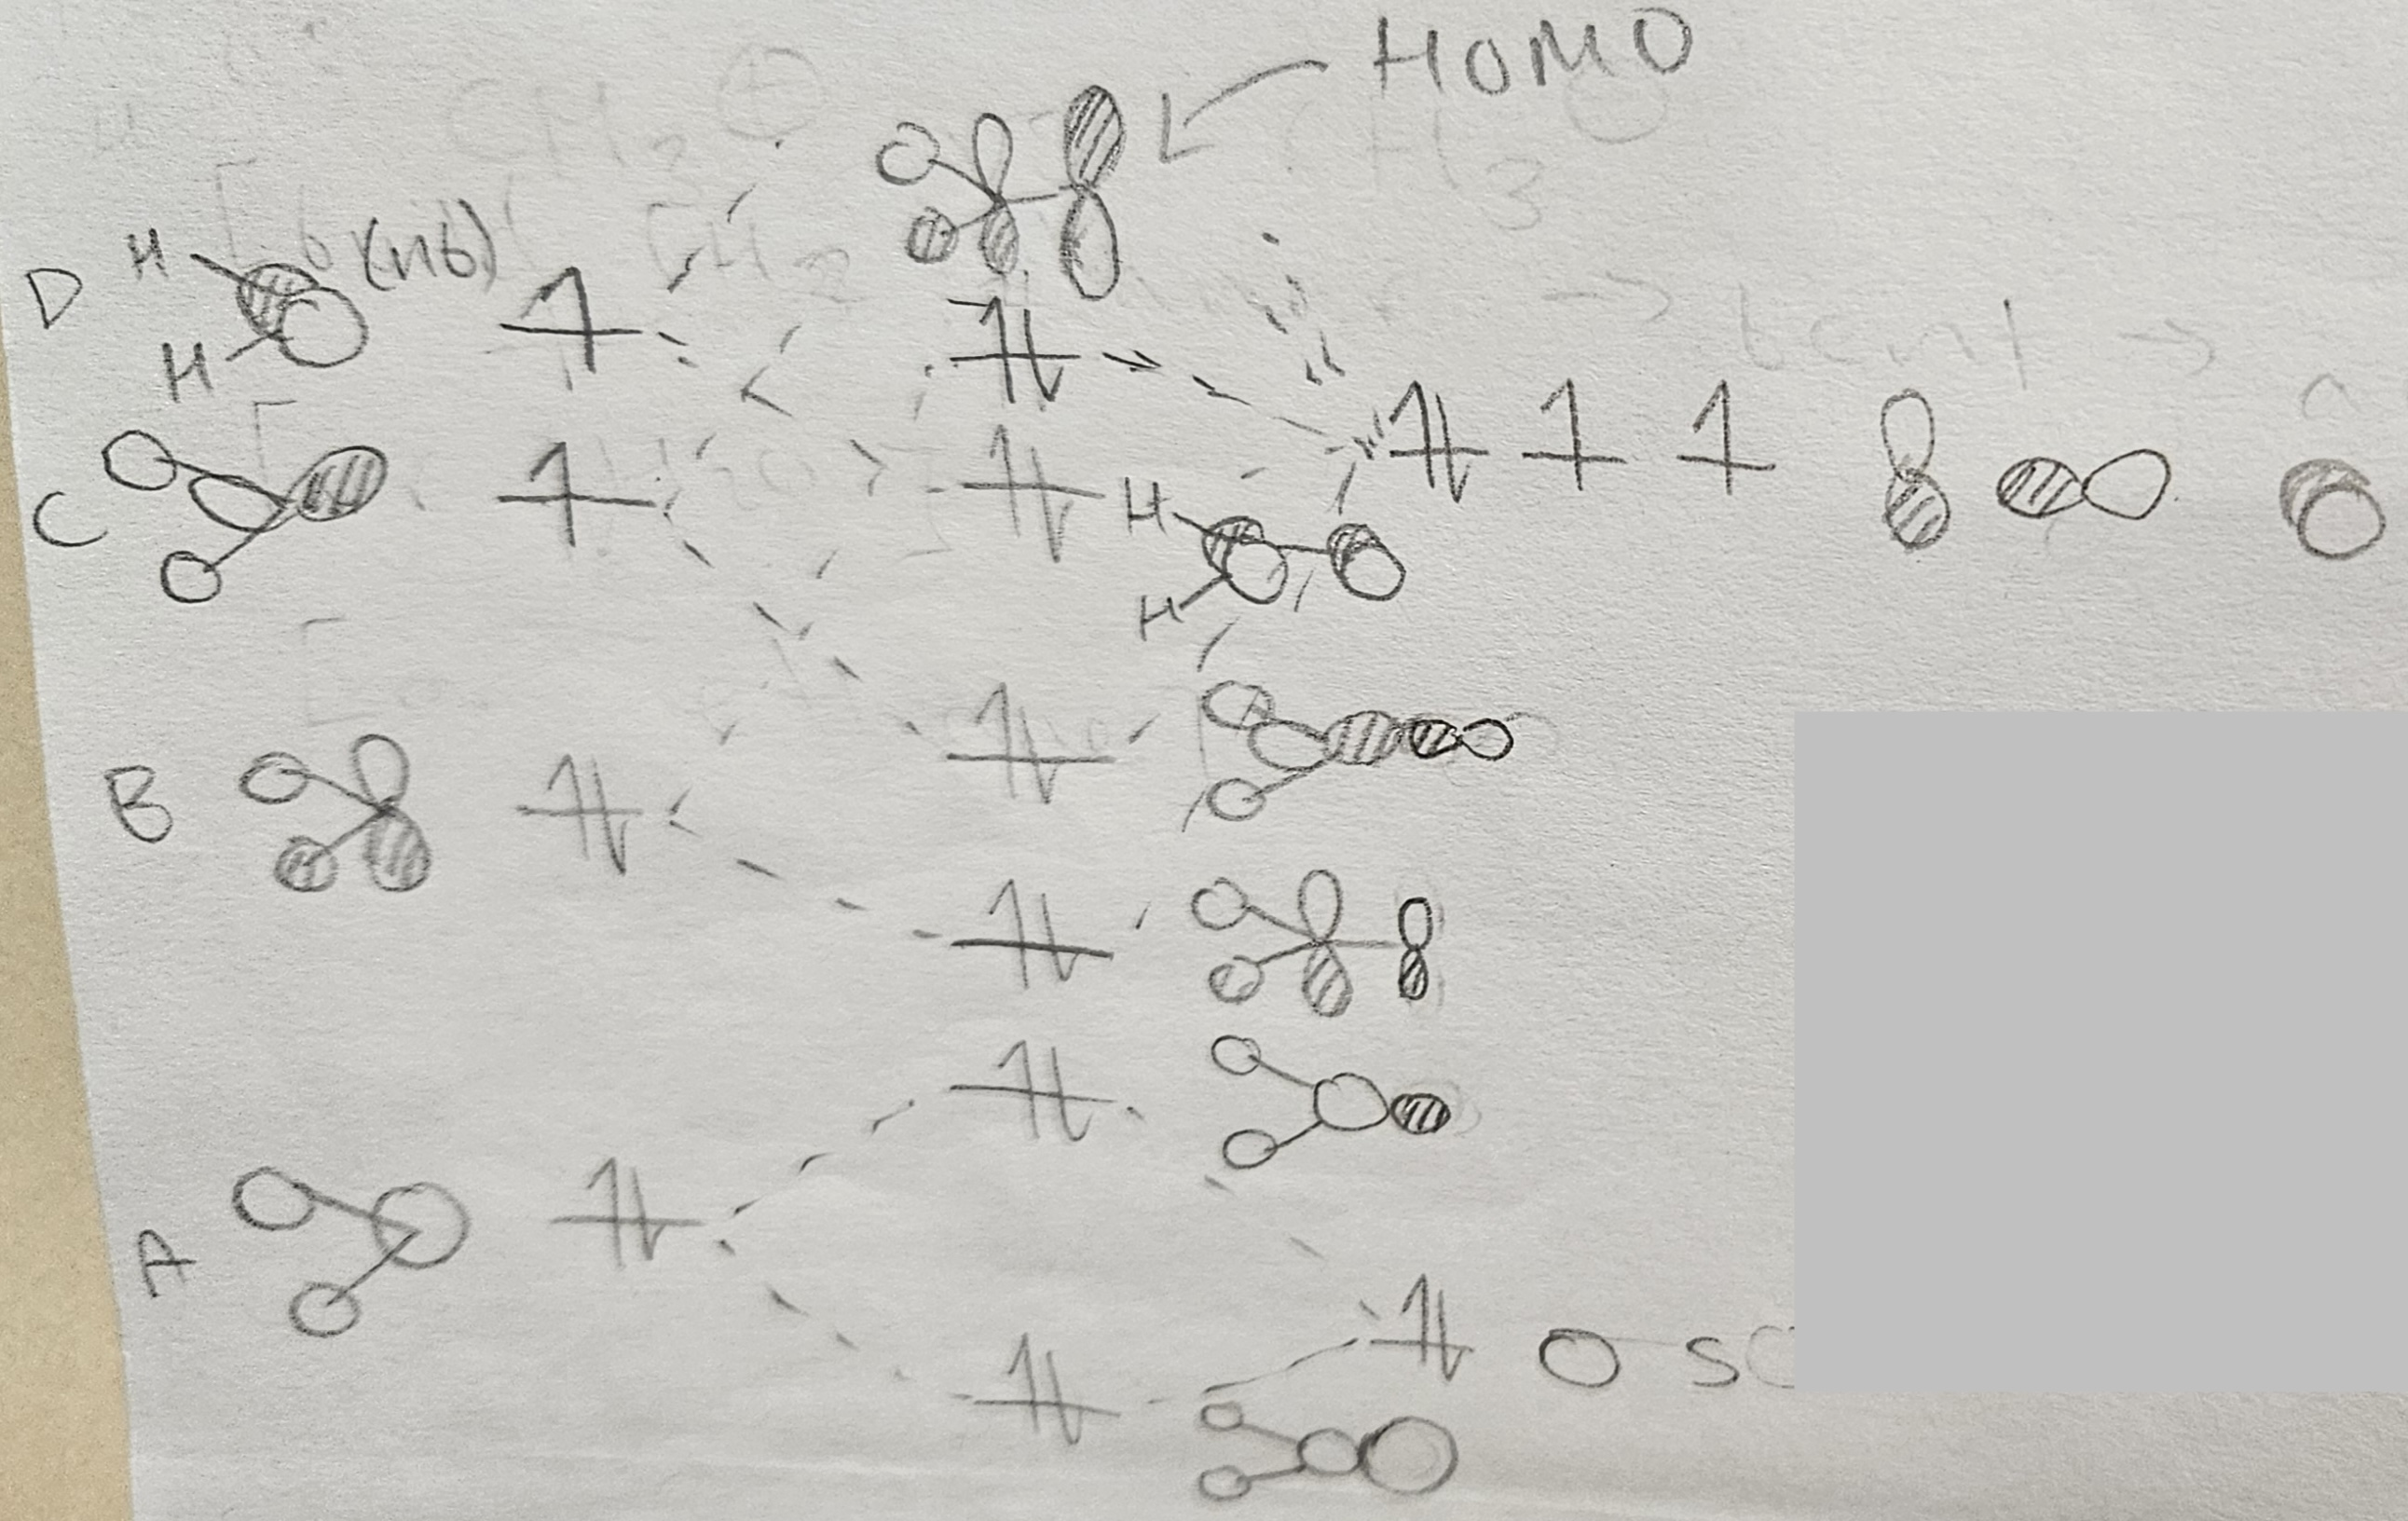
\includegraphics[width=0.6\linewidth]{QmotForm.jpg}
        \caption{QMOT diagram for formaldehyde.}
        \label{fig:QmotForm}
    \end{figure}
    \begin{itemize}
        \item The HOMO has a larger coefficient on \ce{O}; this explains why protonation occurs on \ce{O} and not \ce{C}!
    \end{itemize}
    \item Key takeaway: QMOT diagrams and MO diagrams both make the same predictions about the electronic structure and reactivity of formaldehyde (sanity check).
    \begin{itemize}
        \item Example: They both predict that carbonyls are nucleophilic on oxygen.
        \item Example: Orbital mixing is stronger when orbitals are of similar energy.
        \item Example: Orbital coefficients are larger on an atom when the MO is closer in energy to the AO that originates with that atom.
        \item Example: Orbitals are lower in energy on more electronegative atoms.
        \item Etc.
    \end{itemize}
\end{itemize}




\end{document}